\begin{figure*}%
	\centering%
	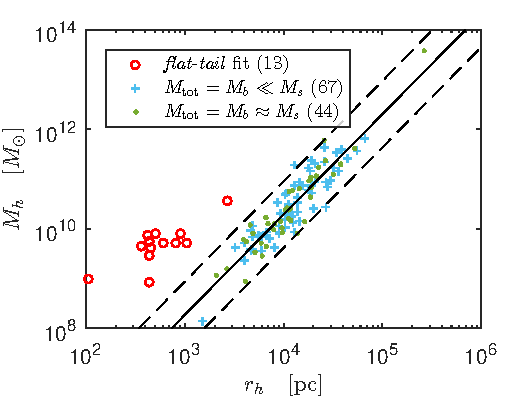
\includegraphics[width=0.33\hsize]{\ROOTPATH/RhMh.pdf}%
	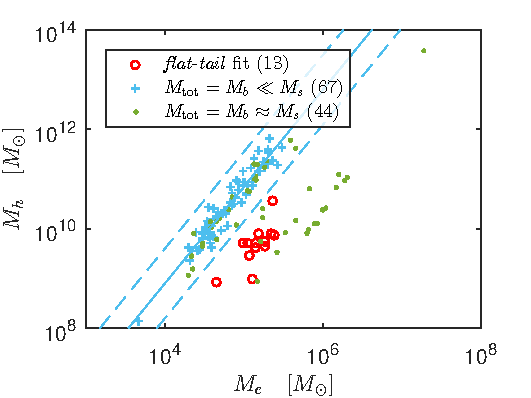
\includegraphics[width=0.33\hsize]{\ROOTPATH/McMh.pdf}%
	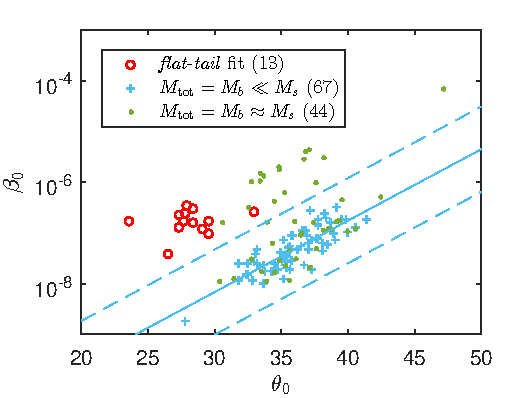
\includegraphics[width=0.33\hsize]{\ROOTPATH/Theta0Beta0.pdf}%
	\caption{Parameter correlations for the best fits of the 50\,keV-RAR model. The galaxy sample in every diagram is classified in three groups: (1) galaxies with appropriate halo information ($M_{\rm tot} = M_b \ll M_s$, dots), (2) with inappropriate halo information ($M_{\rm tot} = M_b \ll M_s$, crosses) and (3) with flat-tail fits which are considered as artifacts (open circles). (\textbf{left}) In the $r_h$-$M_h$ plot we find a correlation with approx. $M_h \sim r_h^2$ (dots and crosses). In contrast to this correlation we may interpret the flat-tail fits as false fits. All of them have in common that the whole dark matter distribution was best-fitted with the flat tail of the RAR model, implying no (or weak) cutoff. Only for one galaxy (NGC4088) we find $\beta_0 \sim 10^{4}$ where pressure effects are not negligible any more. This \textit{outlier} is due to the poor information about the halo where only the cored part without any maxima is available. (\textbf{middle}) Focusing on the $M_c$-$M_h$ plot we clearly identify a distinction between the appropriate (dots) and the inappropriate halo group (crosses). Both follow approx. the relation $M_h \sim M_c^2$ while the appropriate halo group shows a higher diversity. (\textbf{left}) The distinction with the same characteristics is also visible in the $\theta_0$-$\beta_0$ parameter space.}%
\label{fig:param_50keV-RAR}
\end{figure*}